\documentclass{bioinfo}
\copyrightyear{2016} \pubyear{2016}
\access{Advance Access Publication Date: Day Month Year}
\appnotes{Original Paper} 
\usepackage{amsmath, amssymb}
  \allowdisplaybreaks % YEAH!
\newtheorem{thrm}{Theorem}
\usepackage{textcomp}
%\usepackage[
%    colorlinks, linkcolor={blue}, citecolor={blue},
%    urlcolor={red}]{hyperref}
%\renewcommand*{\HyperDestNameFilter}[1]{}
%% Option 1 URW Garamond (free any latex distribution): 
%% ====================
%    \usepackage[urw-garamond]{mathdesign} 
%    \usepackage[T1]{fontenc}
%% Option 2: Classic Garamond (requires .pfb sources)
%% ==========================
%    \usepackage[T1]{fontenc}
%    \usepackage{sabon}
%    \usepackage[italic,defaultmathsizes]{mathastext}
    % mdugm.sty magic bellow --!!!
    \SetSymbolFont{letters}{normal}{OML}{mdugm}{m}{it} 
%% Option 3 (Times via MathTimes Pro)
%% =================================
    %\usepackage[subscriptcorrection]{mtpro}
    %   \DeclareMathSizes{8}{7.15}{5.2}{4.2}
    %\usepackage[mtpcal]{mtpb}
\DeclareMathAlphabet{\txcal}{U}{tx-cal}{m}{n}
\usepackage[scaled=1.1]{rsfso}
\renewcommand*\ttdefault{txtt}
%
%\usepackage{microtype}
%
\newcommand{\wP}{P^\ast}
\newcommand{\wE}{E^\ast}
\newcommand{\wZ}{Z^\ast}
\newcommand{\wt}{\theta^\ast}
\newcommand{\wk}{\psi^\ast}
\newcommand{\whp}{\widehat \pi}
\newcommand{\wAe}{A_e^\ast}
\newcommand{\wAp}{A_p^\ast}
\newcommand{\wBe}{B_e^\ast}
\newcommand{\wBp}{B_p^\ast}
\renewcommand*\copyright{\textcopyright}
\newcommand{\CC}{C\nolinebreak\hspace{-.05em}\raisebox{.4ex}{\tiny\bf
    +}\nolinebreak\hspace{-.10em}\raisebox{.4ex}{\tiny\bf +}} 
\makeatletter

\begin{document}
\firstpage{1}
%\subtitle{}
\title[empirical Bayesian NMF]{An empirical Bayesian approach to
  mutational signature discovery}
\author[Rosales, R. A. and Drummond, R. D.~\textit{et~al}.]{
    R. A. Rosales\,$^{\text{\sfb 1,}\dagger}$, 
    R. D. Drummond\,$^{\text{\sfb 2,}\dagger}$, 
    R. Valieris\,$^{\text{\sfb 2}}$,
    E. Dias-Neto\,$^{\text{\sfb 3}}$,
    I. T. da Silva\,$^{\text{\sfb 2,4}*}$} 
\address{%
   $^{\text{\sf 1}}$Departamento de Computa\c{c}\~ao e
   Matem\'atica, Universidade de S\~ao Paulo, 14040-901 SP, Brazil, 
   $^{\text{\sf 2}}$Laboratory of Bioinformatics and Computational 
   Biology, A. C. Camargo Cancer Center, S\~ao Paulo  01509-010, 
   Brazil, $^{\text{\sf 3}}$Laboratory of Medical Genomics,
   A. C. Camargo Cancer Center, S\~ao Paulo 01509-010, Brazil, 
   $^{\text{\sf 4}}$Laboratory of Molecular Immunology, The
   Rockefeller University, New York, NY 10065, USA\\[1em]
   {\normalsize $^{\dagger}$The authors wish it to be known
     that, in their opinion, the first two authors should be regarded
     as joint First Authors} 
}
\corresp{$^\ast$To whom correspondence should be addressed.} 
\history{Received on XXXXX; revised on XXXXX; accepted on XXXXX} 
\editor{Associate Editor: XXXXXXX} 
\abstract{%
 \textbf{Motivation:} All cancer harbour somatic mutations, ranging 
hundreds to thousands of mutations. Beyond understanding of the
prevalence and types of somatic mutation in cancer genomes, the
causes and features of distinctive mutational process that lead to
neoplastic transformation, however, remain largely unknown.\\
Cancer is an evolutionary process driven by continuous acquisition of
genetic variations in individual cells. The actual identification of
the underlying mutational processes may be central to understanding of
cancer origin and evolution.\\ 
 \textbf{Results:} All cancer harbour somatic mutations, ranging 
hundreds to thousands of mutations. Beyond understanding of the
prevalence and types of somatic mutation in cancer genomes, the
causes and features of distinctive mutational process that lead to
neoplastic transformation, however, remain largely unknown.\\
Cancer is an evolutionary process driven by continuous acquisition of
genetic variations in individual cells. The actual identification of
the underlying mutational processes may be central to understanding of
cancer origin and evolution.\\
 \textbf{Contact:}
%\href{rrosales@usp.br}{\texttt{rrosales@usp.br}},
%\href{rdrummond@gmail.com}{\texttt{rdrummond@gmail.com}},
%\href{rvalieris@gmail.com}{\texttt{rvalieris@gmail.com}},
 itojal@gmail.com\\
\textbf{Supplementary information:} Supplementary data are available  
at \textit{Bioinformatics} online.
}
\maketitle
\section{Introduction}
Cancer emerges as an evolutionary process driven by the continuous
acquisition of heritable genetic variations in individual cells. A set
of acquired mutations allows a growth advantage over its neighbour
cells, thereby triggering the expansion of the tumour
cell clone. The diversity and complexity of somatic mutational
processes in these clones is a conspicuous feature orchestrated by DNA
damage agents and repair processes, including exogenous or endogenous
mutagen exposures, defects in DNA mismatch repair and enzymatic
modification of DNA, \cite{RG}. The actual identification of the
underlying mutational processes is central to an understanding of
cancer origin and evolution, \citealp{RG, AS, HEN}. Most of the
somatic mutations include base substitutions, insertions and deletions
of bases, rearrangements and copy number variations
(CNV).\footnote{\textcolor{red}{Still have to concatenate this with
next paragraph}}


Somatic mutations usually consist of single base substitutions that
fall into one of six possible base changes, namely
\texttt{C:G}$>$\texttt{A:T}, \texttt{C:G}$>$\texttt{G:C},
\texttt{C:G}$>$\texttt{T:A}, \texttt{T:A}$>$\texttt{A:T},
\texttt{T:A}$>$\texttt{C:G} and \texttt{T:A}$>$\texttt{G:C}. According
to \cite{A}, this set may be further enlarged by including the $5'$
and $3'$ neighbouring bases of each substitution site, leading to an 
alphabet $\txcal A$ with 96 trinucleotide mutation types. More
generally, the definition of $\txcal A$ could in principle accommodate
mutations of various other kinds 
%such as indels, rearrangements, copy
%number changes 
and even wider neighbouring contexts. Once $\txcal A$
is properly defined, the counts for the mutations found in $G$
different genomes are assembled into a $K\times G$ matrix $M$ with $K
= |\txcal A|$. A key assumption consists in viewing the counts in $M$
as the additive effect of $N$ mutational processes, each defined as a
$K\times 1$ vector of mutational rates. The later defines what
is known to be as a mutational signature. More precisely, the
mutations across all genomes result as the linear combination of $N$
basis vectors of dimension $K\times 1$, with mixture coefficients
defined by $N$ exposure vectors of dimension $1 \times G$. If the
basis vectors are merged into a $K\times N$ matrix of signatures $P$,
and the coefficient vectors into a $N\times G$ matrix of exposures
$E$, then the data can be simply factored as $M=PE$. An example of
this is shown in Figure~\ref{fig:toyNMF}. 


\begin{figure*}
 \centering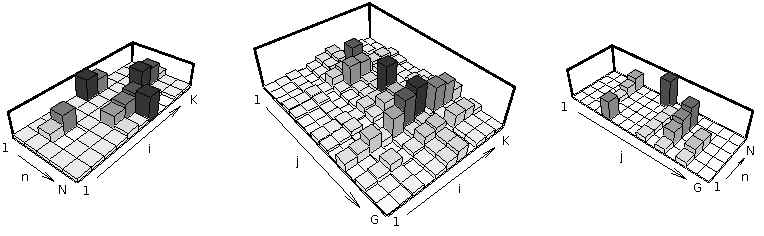
\includegraphics[width=13.5cm]{figs/f_bw_t}
 \caption{\textrm{%
  A factorisation for a mutation counts matrix $M$. The
  mutation matrix shown at the centre is defined over an alphabet with
  $K=11$ symbols, $1 \leqslant i \leqslant 11$, and $G=15$ genomes,
  $1\leqslant j\leqslant 15$. The matrices at the left and the right 
  represent respectively a signature and an exposure matrix $P$ and
  $E$, obtained for a factorisation with rank $N=5$.
  }
 }
\label{fig:toyNMF}
\end{figure*}


For any given a mutation counts matrix there are essentially two
interrelated questions that should be addressed. The first one
concerns the determination of the underlying signatures and exposures
to best account for the observations. The second is related to the
determination of the actual number of signatures $N$. \cite{NCell} and
\cite{A} addressed the first issue by using nonnegative matrix
factorisation (NMF) techniques.  NMF as conceived by \cite{LS} finds
the factors $P$, $E$ that approximately solve the following non-convex
optimisation problem
\begin{equation}
  \label{eqn:NMF}
    \min_{P\geqslant 0,\ E\geqslant 0}\|M - PE\|,
\end{equation}
for a given fixed rank $N$ and an appropriately chosen norm $\|\ \|$.
In order to deal with the second question, \cite{NCell} and \cite{A}
perform the factorisation of the same data for various ranks, namely
for $1 \leq N \leq \min\{K, G\}-1$. The rank is then determined rather 
indirectly by studying the clustering properties of the obtained
factors via a criterion developed by \cite{BTGM} or by using the
residual sum of squares, \cite{HMSG}.

An alternative approach to mutational signature discovery, and to NMF
in general, follows from a statistical interpretation of the problem
posed by (\ref{eqn:NMF}) in which $M$ is assumed to be a random matrix
distributed according to a member of the exponential family
parameterised by $P$ and $E$. The optimisation problem posed by
(\ref{eqn:NMF}), under the norm induced by a specific Bregman
divergence (see \citealp{BMD}), turns to be equivalent to the maximum
likelihood estimation of $P$ and $E$.  For instance, if $M$ is Poisson
distributed with rate $PE$, then the likelihood maximisation with
respect to $P$ and $E$ is equivalent to the minimisation of
(\ref{eqn:NMF}) under the norm defined by the Kullback-Leibler
divergence. The maximisation of a Gaussian likelihood is equivalent to
the minimisation under the Frobenius norm. A key aspect of this
perspective is that it allows to treat the determination of the
factorisation rank $N$ as a model selection problem. The statistical
interpretation was developed by \cite{C}, \cite{FC} and \cite{SWK} in
the general NMF context and then considered by \cite{FICMV} for the
mutational signature application. \cite{FICMV} modelled $M$ as Poisson
distributed and then considered the estimation of $P$ and $E$ by using
an expectation maximisation (EM) algorithm. The number of mutational
signatures where estimated by considering an (unnecessary) saddlepoint
approximation to the Bayesian information criterion
(BIC).\footnote{\textcolor{red}{Finish: state our contribution.}}


Following \cite{FICMV}, our model also takes into account the genome
frequencies of the symbols in $\txcal A$.  These frequencies, known as
the mutation opportunity, enter the model as a weighting matrix $W$, 
such  that the observed mutations are generated at rate $PE\circ W$
with $\circ$ as  Hadamard element wise matrix product.

% Both of these models correspond to the ones initially considered by
% \cite{LS} from the optimisation perspective. The latter is in fact
% the one implemented by \cite{A}. The statistical perspective to NMF
% was observed and then further developed by by \cite{C}, and
% \cite{FC}. A key observation of the statistical approach is that it
% allows to cast the determination of the NMF rank formally as a model
% selection problem. In this regard, \cite{FICMV} considered the 
% estimation of mutational signatures under the Poisson model by
% estimating $P$ and $E$ by an instance of the Expectation
% Maximisation (EM) algorithm, that happens to be be identical to the
% optimisation method in \cite{LS}. The NMF model order is chosen by
% using the Bayesian information Criterion (BIC).

\section{Approach}
\subsection{Hierarchical model}
\subsubsection{Likelihood and latent variables}
Let $p_{in} = (P)_{in}$ be the $i,n$-entry of $P$. Likewise let
$e_{nj} = (E)_{nj}$ and $w_{ij} = (W)_{ij}$.  The mutation counts in
$M$ are assumed to be independent and Poisson distributed random
variables with rates $PE\circ W$, that is, we assume $M_{ij}$ to be
Poisson with rate $(PE)_{ij}(W)_{ij} = w_{ij}\sum_{n=1}^N
p_{in}e_{nj}$. For a given sample of $M$, say $m$, this formulation is
sufficient to define the likelihood function $\mathcal L(\theta; m)$
if one identifies the matrices $P, E$ as model parameters $\theta$,
for $\theta \in \Theta = \mathbb R_+^{K\times N}\times \mathbb
R_+^{N\times G}$. We observe that the opportunities, when available,
are regarded as known parameters and in this sense the likelihood is
is  defined by the function $\mathcal L(\theta, W; m)$. To simplify 
notation we omit any further reference to $W$. A full expression
for $\mathcal L(\theta; m)$ is presented in ($s_1$).


This relatively simple model allows for a latent variable
representation in which the observed counts are expressed as the sum
of $N\geqslant 1$ independent Poisson variables
\begin{equation}
  \label{eqn:latent_representation}
   M_{ij} = Z_{i1j} + Z_{i2j} + \ldots + Z_{iNj},
\end{equation} 
each with rate respectively equal to $p_{in}e_{nj}w_{ij}$. This
description is an immediate consequence of the properties of sums of
independent Poisson random variables. Biologically, this accounts for
the observation that the total number of mutations of a specific type,
say $(i,j)$, arise as the linear combination of $N$ mutational
processes $Z_{inj}$, $n = 1, \ldots, N$. From a statistical
perspective, (\ref{eqn:latent_representation}) enables a data
augmentation scheme that becomes instrumental for a Bayesian treatment
to NMF. As observed by \cite{C}, this allows the implementation of
several powerful techniques such as the Expectation Maximisation (EM)
algorithm, Markov chain Monte Carlo (MCMC), and variational Bayesian
approximations.  Our statistical approach to NMF fully exploits the
data augmentation scheme provided
by~(\ref{eqn:latent_representation}).  Hereafter let $Z = \{Z_{inj}:
1\leqslant i\leqslant K, 1\leqslant n \leqslant N, 1\leqslant
j\leqslant G\}$, and $z$ denote a generic value for $Z$.


\subsubsection{Priors and hyperpriors} 
We consider conjugate priors for the matrices $P$ ans $E$ by modeling
each of their entries as being independent Gamma distributed random
variables. Specifically, $p_{in}$ is Gamma distributed with shape
$\alpha_{in}^p + 1$ and rate $\beta_{in}^p$ for $\alpha_{in}^p
\geqslant 0$, $\beta_{in}^p \geqslant 0$. Likewise, $e_{nj}$ are Gamma
with shape $\alpha_{nj}^e+1$ and rate $\beta_{nj}^e$ with
$\alpha_{nj}^e \geqslant 0$, $\beta_{nj}^e \geqslant 0$. Shape
parameters are shifted by 1 to ensure bounded values for the Gamma
densities\footnote{\textcolor{red}{RD: we need to explain this.  That
is, why do we have to avoid a `singularity' near the origin?}}. Let
$A_p$ and $B_p$ be $K\times N$ matrices respectively with entries
$\alpha_{in}^p$ and $\beta_{in}^p$ and $A_e$, $B_e$ be $N\times G$
matrices with elements $\alpha_{nj}^e$ and $\beta_{nj}^e$, and then
let $\psi = (A_p, B_p, A_e, B_e)$.


A further hierarchy in our model is set by considering the
distributions for the hyperparameters $\psi$. By conjugancy to the
prior, we define the entries of $B_p$ as being independent and
distributed according to a common Gamma distribution with shape and
rate $a_p > 0$, $b_p > 0$. Similarly, the elements of $B_e$ are Gamma
distributed with the same shape $a_e>0$ and rate $b_e>0$. The
situation for the matrices $A_p$ and $A_e$ is however different. While
a Gamma distribution for the entries of $A_p$ and $A_e$ is conjugate
to the Gamma prior (see \citealp{M}), the resulting full conditional
distribution necessary in order to draw inferences about $A_p$ and
$A_e$ does not has a standard form.  This fact has long been
recognized in the Poisson hierarchical model (\citealp{GMS93}) and may
be dealt with by choosing any parametric family of
distributions with the appropriate support. Here we consider the
elements of $A_p$ and $A_e$ as independent and exponentially
distributed with rates $\lambda_p > 0$ and $\lambda_e > 0$.  Define
$\eta$ as the vector of hyperprior parameters $\eta = (a_e$, $b_e$,
$a_p$, $b_p$, $\lambda_p$, $\lambda_e) \in \Lambda = (0, \infty)^6$.
% $\psi \in \Psi = \mathbb R_+^{K\times N}\times \mathbb R_+^{N\times
% G}\times \mathbb R_+^{K\times N}\times\mathbb R_+^{N\times G}$ and 
% $z \in \txcal Z = \mathbb Z_+^{K\times N\times G}$.

\subsection{Bayesian treatment}
We follow an empirical Bayesian approach in which the parameters
$\theta$, the hyperparameters $\psi$ and the hyperprior parameters
$\eta$ are all estimated from the data.  Inferences about the
mutational signatures and their exposures are driven by the
conditional posterior distribution for the NMF model by combining
Markov chain Monte Carlo (MCMC) and EM techniques as encouraged by
\cite{C01}. Specifically, for a given value of $\eta$ we consider a
Metropolized Gibbs sampler targeted towards the conditional posterior
$\pi(\theta|M, \eta)$. This entails the iterative generation of a
sequence of samples $\big(Z^{(r)}, \theta^{(r)}, \psi^{(r)}\big)$, $r
\geqslant 1$, from the set of full conditional distributions
\begin{gather*}
   Z^{(r+1)} \sim \pi(Z| \theta^{(r)}, \psi^{(r)}, M, \eta), \qquad
   \theta^{(r+1)} \sim \pi(\theta| Z^{(r+1)}, \psi^{(r)}, M, \eta), \\
       \text{and}\quad
   \psi^{(r+1)} \sim \pi(\psi| Z^{(r+1)}, \theta^{(r+1)}, M, \eta).
\end{gather*}
These samples are used to update the value of $\eta$ via a
stochastic EM step and the later is then used to draw a subsequent
sequence of samples for $Z$, $\theta$ and $\psi$. The successive iteration of these steps defines a 
convergent sequence $\big(\eta^{(u)}\big)$, $u \geq 1$, leading
towards the estimate $\hat\eta = \eta^{(U)}$ for
sufficiently large $U$. A final set of MCMC samples for $Z$, $\theta$
and $\psi$ drawn by conditioning on $\hat\eta$ allow for the
following Monte Carlo estimate
\begin{equation}
 \label{eqn:MCEM_estimate}
   \widehat{\pi}(\theta|M, \hat\eta)
 = 
   \frac{1}{R}\sum_{r=1}^R \pi(\theta|Z^{(r)}, \psi^{(r)}, M,
   \eta^{(U)})
\end{equation}
of the posterior $\pi(\theta|M, \eta)$.


The samples for $\theta$ are used to compute point estimates for
$\theta$ and related posterior statistics. In particular, estimates
for the mutation signatures and their exposures are computed as
$\widehat P = R^{-1}\sum_{r=1}^R P^{(r)}$ and $\widehat E =
R^{-1}\sum_{r=1}^R E^{(r)}$. Posterior variances or coverage intervals
for $P$ and $E$ also be obtained from the samples $\theta^{(r)}$. 


Details about the Gibbs sampler are relatively standard and are
included in Section 2 of the supplementary material. The following
section details the Monte Carlo EM approach.

\subsubsection{MCMC EM}\label{sec:MCMCEM}
For a given data sample $m$ and $Z = z$, direct use of Bayes theorem 
allows to  express the the marginal likelihood for $\eta$, i.e. the
function $\mathcal L: \Lambda \to \mathbb R$ induced by $\eta 
\mapsto p(M=m|\eta)$, as
\begin{equation}
  \label{eqn:margLik}
  \mathcal L(\eta; m) 
  = \frac{\mathcal L(m, z, \theta, \psi\,|\,\eta)}{\pi(z,
      \theta, \psi|m, \eta)}
\end{equation}
with $\mathcal L(\eta; m, z, \theta, \psi)$ 
defined as being equal to the distribution $p(M=m$, $Z=z$, $\theta$,
$\psi|\eta)$ but considered as a function of $\eta$.  This function
can be evaluated by observing the conditional decomposition
\[
   \mathcal L(\eta; m, z, \theta, \psi) 
  = 
   p(M=m, Z=z|\theta) p(\theta|\psi)p(\psi|\eta), 
\]
where $p(\theta|\psi)$ and $p(\psi|\eta)$ stand respectively for the
prior and the hyperprior distributions and $p(M=m, Z=z|\theta)$
is the complete data likelihood. An expression for the later is given
by ($s_2$) in the supplementary material. Taking logarithms and
integrating with respect to the posterior distribution $\pi(Z, \theta,
\psi|m, \eta)$ with $\eta = \eta_0$ at both sides of
(\ref{eqn:margLik}) gives 
\begin{align*}
   \mathbb E\big[\ln\mathcal L(\eta; m) \big| \eta_0\big] 
  =& 
  \mathbb E\big[\ln\mathcal L(\eta; m, Z, \theta, \psi)
    \big|  \eta_0\big]\\ 
  &-
  \mathbb E\big[\ln \pi(Z, \theta, \psi\,|\,m,\eta)\big| \eta_0\big].
\end{align*}  
This expression is the basic identity on which the EM algorithm is
built and justifies therefore the convergence of the sequence
\begin{equation}
 \label{eqn:EofMCEM}
  \eta^{(u+1)} = \underset{\eta\,\in\, \Lambda}{\text{arg max}}\, 
  \mathbb E\Big[\ln\mathcal L(\eta; m, Z, \theta, \psi)\big|
  \eta^{(u)}\Big], 
  \quad u\geqslant 0,
\end{equation}
towards the maximum likelihood estimate of $\eta$ for any $\eta^{(0)}
= \eta_0  \in \Lambda$. The integral involved in the above expectation
cannot be computed directly but it may be estimated via Monte Carlo,
leading to the sequence 
\begin{equation}
 \label{eqn:MCEM}
   \hat\eta^{(u+1)}
 = 
    \underset{\hat\eta^{(u)}\,\in\,\Lambda}{\text{arg max}} 
   \bigg\{
    \frac{1}{R}\sum_{r=1}^R 
      \ln\mathcal L\Big(\hat\eta^{(u)}; m, Z^{(r)}, \theta^{(r)},
      \psi^{(r)}\Big)
   \bigg\}.
\end{equation}
The maximisation steps involved in (\ref{eqn:MCEM}) are relatively
simple to implement and further detailed in Section 3.1 of the
supplementary material.


The procedure described is valid because the sampler developed
throughout generates $\big(Z^{(r)}, \theta^{(r)}, \psi^{(r)}\big)$
approximately from the posterior distribution that is actually used to
define the expectation in (\ref{eqn:EofMCEM}), see for example
\cite{FM}. This rises however the issue as to in what sense
$\widehat\pi(\theta|M, \hat\eta)$ defined by (\ref{eqn:MCEM_estimate})
can be regarded as an estimate for $\pi(\theta|M, \eta)$. The answer
to this is provided by the following result. Let $f(\theta|M, \eta)$
be the density of the posterior distribution $\pi(\theta|M, \eta)$.


\begin{thrm} For any measurable set $B\subseteq \Theta$,
 $\widehat\pi(B|M,\hat\eta)$ converges in total variation
towards $\pi(B|M,\eta)$ as $R, U \to \infty$, that is
\[
   \lim_{U,\ R\to\infty}
   \sup_{B}
    \bigg|
     \int_B
      % \frac{1}{R} \sum_{r=1}^R \pi(\theta|M, \psi^{(r)}, Z^{(r)}, 
      %    \hat\eta^{(U)}) 
     \Big[
       \widehat \pi(\theta|M, \hat\eta) - f(\theta|M,\eta)
     \Big]\ d\theta
    \bigg|
   = 0.
\]
%\[
%    \lim_{R,\ u\to\infty}
%     \big|
%       \widehat\pi(\, B|M, \hat\eta) - \pi(\, B|M,\eta)
%     \big|
%   =
%    0,
%\]
%where converge is with respect to the total variation norm. 
\end{thrm}

The proof to this is included in Section 3.2 of the accompanying 
supplementary material.

\subsection{Parameter estimation}
The algorithm to estimate $\eta$ and generate the samples for $(Z,
\theta, \psi)$ conditionally upon the estimate for $\eta$ proceeds as 
follows. 
\begin{enumerate}
\item[\textbf{1}.] Set $u = 0$ and initialise $\eta^{(0)}$ as
  $\eta^{(0)} = (1, \ldots, 1)$.
\item[\textbf{2}.] Initialise $Z^{(0)}$, $\theta^{(0)}$, $\psi^{(0)}$
  by sampling according to the hierarchical model, that is
  \begin{align*}
     &\psi^{(0)} \sim p(\psi | \eta^{(0)}) &\ 
        &\text{hyperprior}\\ 
     &\theta^{(0)} \sim p(\theta | \psi^{(0)}) &\ 
        &\text{prior}\\
     &Z^{(0)} \sim p(Z, M|\theta^{(0)}) &\ 
        &\text{complete data likelihood}
  \end{align*}
  Alternatively, the values for $\theta^{(0)}$ may be set by solving 
  (\ref{eqn:NMF}) via the NMF package from within R, see
  \citealp{GS}.
\item[\textbf{3}.] Iterate the Gibbs sampler to generate the sequence
 $\big(Z^{(r)}, \theta^{(r)}, \psi^{(r)}\big)$, $r = 1, \ldots, R$.
\item[\textbf{4}.] Update $\hat\eta^{(u)}$ with the Monte Carlo EM
formula in (\ref{eqn:MCEM}) and set $u = u+1$. Return to step
\textbf{3} until $\big\|\hat\eta^{(u)} - \hat\eta^{(u-1)}\big\|_\infty  
\leqslant 0.05$ or $u > 4000$. 
\item[\textbf{5}.] Set $\hat\eta = \hat\eta^{(u)}$ and then iterate
  the Gibbs sampler to obtain the final sequence of samples
  $\big(Z^{(r)}, \theta^{(r)}, \psi^{(r)}\big)$, $r=1, \ldots,
  R$. 
\end{enumerate}

\subsection{Model selection}
The samples for $\theta$ generated by the last iteration of the
MCMC/EM analysis is considered for the estimation of the number 
of mutational signatures $N$. To this end, for each $N$ we consider
the set of BIC values
\[
  \text{BIC}\big(\theta^{(r)}_N\big) = 2\ln\mathcal L\big(m;
    \theta^{(r)}_{N}\big) - N(G+K)\ln G, \qquad r =1, \ldots,
    R
\]
with $\theta^{(r)}_N$ as the sequence of signature and exposure 
samples obtained while analysing the  data with $N$
signatures. Contrary to previous approaches, the evaluation of the BIC
does not requires any further approximation because the likelihood
$\mathcal L(\theta^{(r)}_N; m)$ is directly available.

\subsection{Differential Exposure Score and Classification}
\textcolor{red}{RD: This may be the place to explain your 
ideas.} 


\section{Methods}
\subsection{Data} The data set containing 183916 somatic point
mutations from 21 breast cancer genomes was obtained from
\verb+ftp://ftp.sanger.ac.uk/+ \verb+pub/cancer/Nik-ZainalEtAl+, by
following the instructions in Table S1 in~\cite{NCell}. Single base 
substitutions where mapped onto trinucleotide sequences by considering
the $5'$ and $3'$ neighboring bases in order to construct a $96\times
21$ matrix of mutation counts $M$. 
%\footnote{IT, RD, RV: What is the
%appropriate way to reference this?  Some papers (by
%Nik-Zainal/Alexandrov) point to COSMIC
%(\verb+http://www.sanger.ac.uk/genetics/CGP/cosmic+), but I have not
%been able to find the data there! The ftp link here was found in
%Table S1 of \cite{NCell}. DO CHECK.}. 
The $(i,j)$-th element of the opportunity matrix was computed as the
cumulative sum of the number of times that the $i$-th symbol of
$\txcal A$ occurs in the $j$-th genome. This frequency was then
multiplied by the CNV information found in the data set by
\cite{NCell}.


Synthetic data sets mimicking real observations were assembled by
taking a group of four mutational signatures commonly found in 
breast cancer genomes, namely the signatures 1, 2, 3 and 13 described   
in the Catalogue  of somatic  mutations in cancer,
\verb~http://cancer.sanger.ac.uk/cosmic/signatures~.
\footnote{\textcolor{red}{RD:explain how do we simulate $E$ and how do
    we add extra noise}}. 
Signature 1 is the result of an endogenous mutational process
initiated by spontaneous deamination of 5-methylcytosine and has been
found in most cancer samples. Signature 2 is related to the activity
of the AID/APOBEC family of cytidine deaminases. Signature 3 is
associated with failure of DNA double-strand break-repair by
homologous recombination and is strongly associated with
germline and somatic BRCA1 and BRCA2 mutations in breast cancer.
Signature 13 causes predominantly \texttt{C>G} mutations.


\subsection{\texttt{signeR}} Describe R's package 
source destination. Mention that is has been optimized in
\CC. A detailed explanation about how to install, run, etc is 
presented as supplementary material. 

\section{Results}
\subsection{21 breast cancer data}
Our analysis of the 21 breast cancer data revealed 5 biologically
distinct signatures (Figure~\ref{fig:bcancer}.A). These results agree
well with existing knowledge. Signatures $S_1$ and $S_5$ are
attributed to activity of the  APOBEC family of cytidine
deaminases. Signature $S_2$ is associated with a process initiated by 
the spontaneous deamination of 5-methylcytosine and it correlates with 
age of cancer diagnosis. Signature $S_3$ is associated 
with failure of DNA double-strand break-repair by homologous
recombination.  Signature $S_4$ is of unknown 
aetiology. The two most highly exposed signatures, namely $S_1$ and
$S_2$ were also found in \cite{FICMV} and $S_1$, $S_2$, $S_3$, and 
$S_5$ were described by \cite{A}. The determination of the number of 
signatures is based on the median of the BIC values obtained by
varying $N$ from 1 to 95\footnote{\textcolor{red}{RD: please set the
    right upper limit for $N$ considered by \texttt{signeR}}}.
 Figure~\ref{fig:bcancer}.B presents the box
plots obtained at each model rank.

The results for the differential exposure analysis are shown in 
Figure~\ref{fig:bcancer}.C. Specifically, we considered samples
with and without germinative mutations in BRCA1 and BRCA2 genes, thus
providing a better understanding of how germline mutation status may
lead to distinctive mutational patterns. The protein products of BRCA1
and BRCA2 plays a role in maintaining genomic stability and are
involved in a variety of cellular processes such as damage signaling
and DNA repair (\citealp{LY}). Disruption of such processes often
leads to a rapid accumulation of somatic mutations in cancer
genomes. DES highlights four mutational signatures
(Figure~\ref{fig:bcancer}: $S_3$-$S_5$), two of these are associated
with inactivating mutations in BRCA1/BRCA2 (Figure 1: S3) and
implicate to activity of APOBEC (Figure 1: S1,S3) respectively. Taken
together, this finding is consistent with existing knowledge and
thereby may help explain the failure in the response to DNA damage by
homologous recombination in BRCA-defective breast cancer. Based on
this, we conclude that our DES method allows reveal features into
genotype-phenotype relationships between groups of interest.
 

\begin{figure*}
  \centering
  \begin{tabular}{c}
   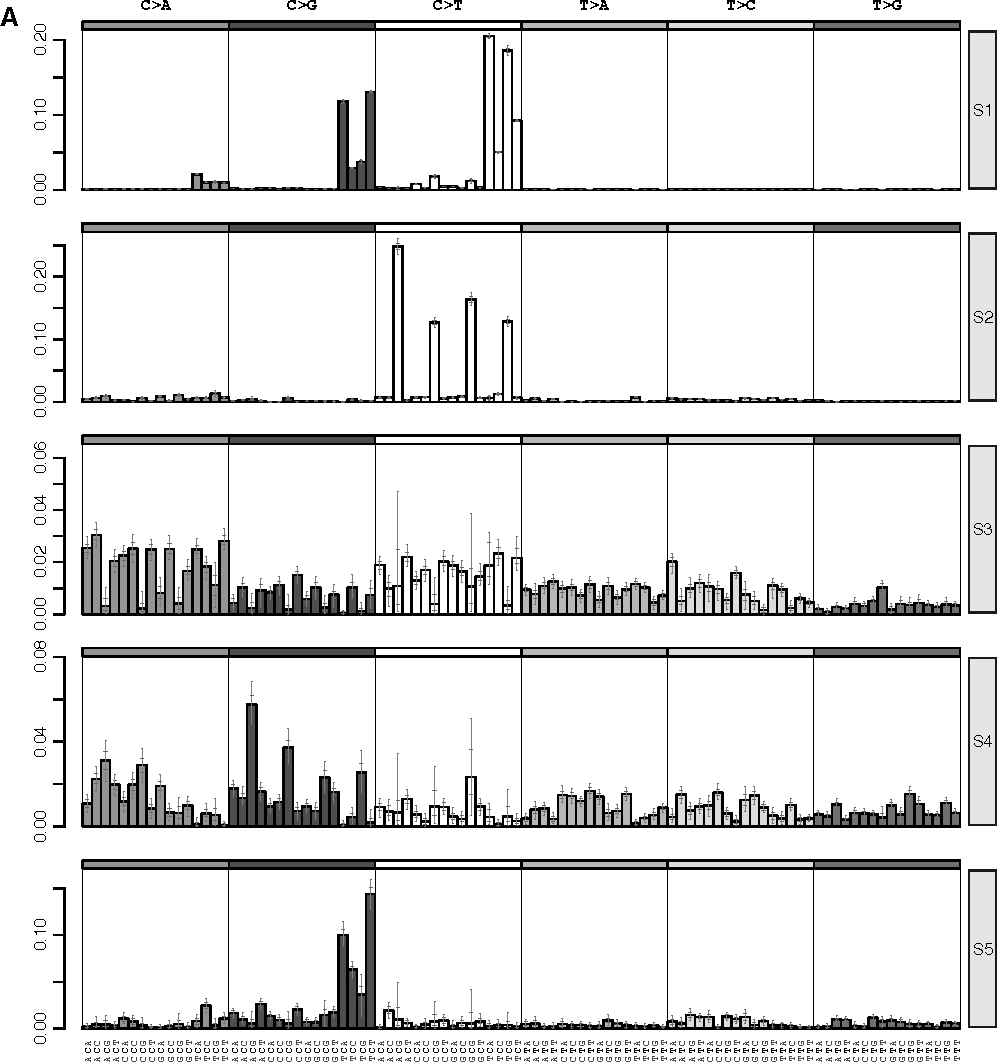
\includegraphics[width=13cm]{figs/Signatures_5_com_Opp_bw}
  \\
   \begin{tabular}{ccc}
    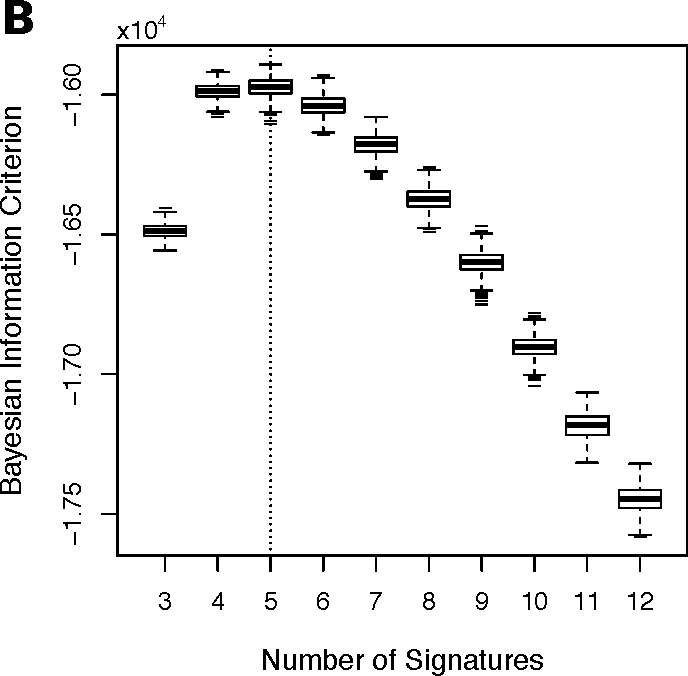
\includegraphics[width=5.5cm]{figs/BICs_21bc_with_Opportunity_5_3to12}
   &
     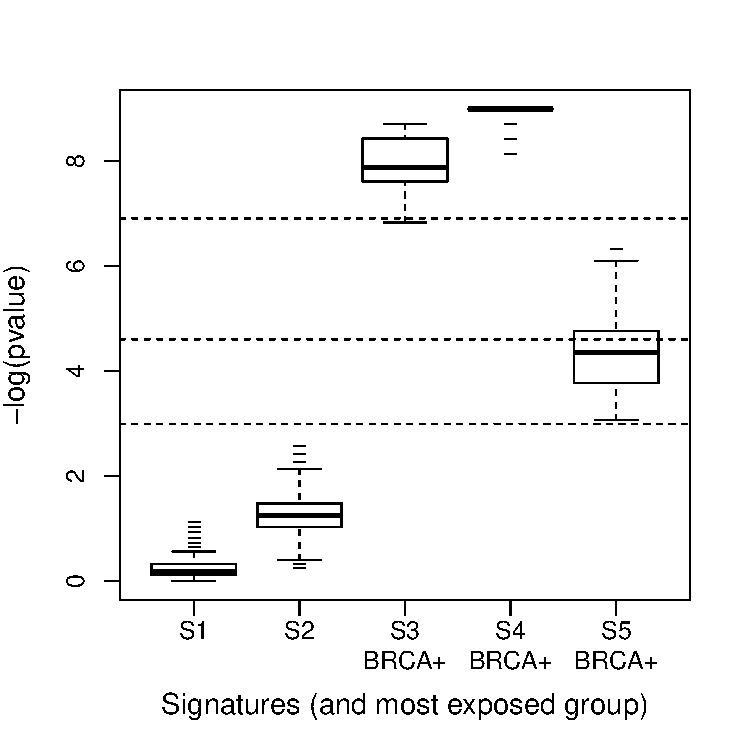
\includegraphics[width=5.5cm]{figs/Diffexp_boxplot_21bc_com_Opp_b2}
   &
     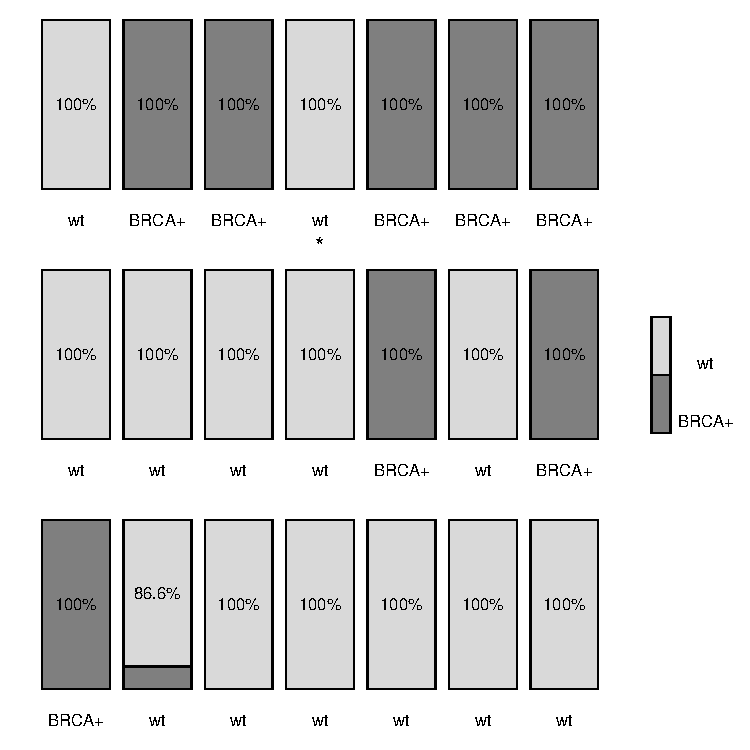
\includegraphics[width=5.5cm]{figs/Classific_result_with_Opp_5b}
   \end{tabular}
 \end{tabular}
 \caption{\textrm{%
     Results for the 21 breast cancer data. A presents the five
    signatures obtained for the highest NMF model rank according to the
BIC score presented in B. Signatures are labelled according to the
order induced by the total signature exposure defined as $\hat e_n =
\sum_{j} \hat e_{nj}$, with $S_1$ being the most exposed
signature. Mention the rescaling so that sum of bars equals 1?
Mention what the small horizontal levels are: posterior marginal
estimates for each component media, and *, *, * percentiles. B: values
for the BIC$(\theta^{(r)}_N)$, $1 \leq r \leq R$ obtained at various
NMF ranks, $N$. C: Differential exposure scores: mention that the
dashed lines are located at the significance levels 0.05, 0.01 and
0.001. D: Classification \textcolor{red}{RD: please explain briefly.}
  }
 }\label{fig:bcancer} 
\end{figure*} 

The analysis of the 21 breast cancer data is summarised in
Figure 2. Describe the signatures: say what the different
bars present (I mean the median, etc...). Compare this to figure * in
*. Explain the model selection result.
 
Explain the differential exposure result. Focus on biology, importance
of this from a biological perspective.

Include the classification result.

\subsection{Simulation study}
Mention the results with the simulated data: focus on the robustness
of our method. Observe that this data set is rather challenging from
an inferential point of view because of the similarity of two of the 
 signatures considered (see signatures $S_*$, and $S_{**}$ in Figure
 S*).



\section{Discussion}
The idea that many cancers acquire a mutator phenotype at different 
intensities is well accepted. Therefore, the ability to detect 
mutational signatures may provide insights about the development of
tumours. Here, we have outlined signeR, it employs a different and 
novel approach to deciphering mutational signatures, and featuring a
number of advantages when compared with others approaches. First, it
xxx $\ldots$ Second, xxx and Third $\ldots$ 


Our method is robust. It requires minimal intervention from part of
the user, but it also allows the incorporation of prior information
into the modelling. This justifies in part the empirical
approach. Mention that this reduces considerably the number of
parameters that have to be specified: from $2(KN+NG)=1170$ hyper
parameters down to 6.


Our method considers the model selection problem robustly. Elaborate
on the model selection problem to NMF --there is space for
improvement. Close.


\section*{Funding}
This work was partially supported by Funda\c{c}\~ao de Apoio a
Pesquisa do Estado de S\~ao Paulo (FAPESP), grant $\ldots$. 
\vspace*{-12pt}
 
%\bibliographystyle: natbib, achemnat, plainnat, abbrv, plain
\bibliographystyle{bioinformatics} 
\bibliography{bnmf}
\end{document} 

%%% Local Variables:
%%% mode: latex
%%% TeX-master: t
%%% End:


At hyperpriors section:

Maybe we have to justify why all this was made. The reason is to
reduce the dependency on a large number of free hyperparameters for
the model choice approach, i.e. the prior depends upon the
values of the hyperparameters if we don't integrate them out: for
$N=5$, $G=21$, $K=96$ we have $2(KN+NG)=1170$ (hyper)parameters to
set. With the hierarchical model, we are able to reduce the free
parameters down to 6.